\section{Theoretische Grundlagen}
\subsection{Entstehung und Nachweis von Röntgenstrahlung}
Als Röntgenstrahlen wird elektromagnetische Strahlung mit Photonenenergien höher als bei UV-Licht bezeichnet. Um zwischen Röntgen- und $\gamma$-Strahlung unterscheiden zu können, ist die Entstehung der jeweiligen strahlung wichtig. $\gamma$-Strahlung entsteht durch Übergänge im Atomkern während Röntgenstrahlung durch hochenergetische Übergänge in der Atomhülle oder durch Bremsstrahlung entsteht. Je nach Entstehung kann die Röntgenstrahlung also ein kontinuierliches Spektrum (durch Bremsstrahlung) oder ein diskretes Spektrum (durch Übergänge in Atomhülle) haben.\\ \\
Um mit der Röntgenstrahlung Materialien untersuchen zu können ist es wichtig, die Entstehung des diskreten Spektrums theoretisch nachvollziehen zu können. Dabei reicht es aus, Atome mit dem Schalenmodell zu beschreiben. Trifft ein Elektron mit ausreichender Energie auf ein Atom kann es ein Elektron auf ein höheres Niveau anregen oder sogar Ionisieren. Damit das Atom wieder in den Grundzustand gelangt wird die entstandene Lücke durch ein Elektron aus einer höheren Schale aufgefüllt. Dieses emittiert bei dem Übergang elektromagnetische Strahlung. Wird ein Elektron aus der ersten Schale herausgelöst und durch ein Elektron aus einer höheren Schale ersetzt, spricht man bei der emittierten Strahlung von den $K$-Linie (siehe Abb. \ref{fig:k_linien}). Äquivalent sind die $L$-, $M$-,... Schalen definiert, bei denen zunächst ein Elektron aus der ersten, zweiten, ... Schale herausgelöst wird. Durch die Feinstruktur werden die Linien in weitere Linien aufgespalten.
\begin{figure}[h]
  \centering
  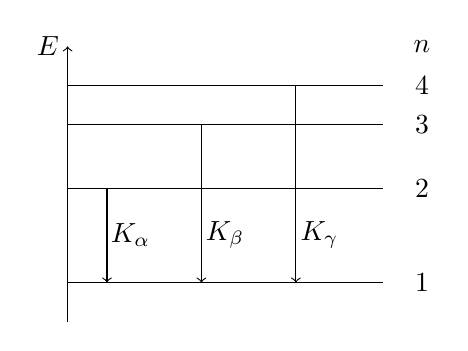
\begin{tikzpicture}
    \draw [->] (0,-3.5)--(0,0);
    \draw (-0.25,0) node {$E$};
    \draw (0,-3)--(4,-3);
    \draw (4.5,-3) node {$1$};
    \draw (0,-8*1/4+0.2)--(4,-8*1/4+0.2);
    \draw (4.5,-1.8) node {$2$};
    \draw (0,-8*1/9-0.1)--(4,-8*1/9-0.1);
    \draw (4.5,-8/9-0.1) node {$3$};
    \draw (0,-8*1/16)--(4,-8*1/16);
    \draw (4.5,-0.5) node {$4$};
    \draw (4.5,0) node {$n$};
    \draw [->](0.5,-1.8)--(0.5,-3);
    \draw (0.8,-2.4) node {$K_\alpha$};
    \draw [->](1.7,-8/9-0.1)--(1.7,-3);
    \draw (2,-2.4) node {$K_\beta$};
    \draw [->](2.9,-0.5)--(2.9,-3);
    \draw (3.2,-2.4) node {$K_\gamma$};
  \end{tikzpicture}
  \caption{$K$-Linien des charakteristischen Spektrums}
  \label{fig:k_linien}
\end{figure}

Nachgewiesen werden kann die Röntgenstrahlung wegen ihrer hohen Photonenenergie durch die ionisierende Wirkung. In dem Versuch wird dabei ein Zählrohr verwendet (siehe Abb. \ref{fig:rohr}). Trifft die Röntgenstrahlung auf das gas in dem Zylinder wird dieses ionisiert. Die freien Elektronen bewegen sich dann zur Anode und können auf dem Weg weitere Atome ionisieren. Die so verursachte Elektronenlawine erzeugt einen messbaren Strom $I$. 

\begin{figure}[h]
  \centering
  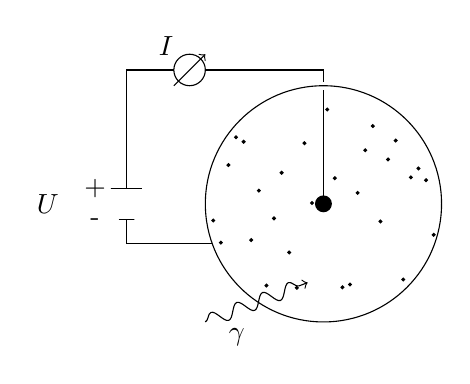
\begin{tikzpicture}
    \draw (0,0) circle (1.5);
    \draw [black, fill=black] (0,0) circle (0.1);
    \draw (0,0)--(0,1.45);
    \draw (0,1.55)--(0,1.7)--(-1.5,1.7);
    \draw (-1.7,1.7) circle (0.2);
    \draw [->] (-1.9,1.5)--(-1.5,1.9);
    \draw (-2,2) node {$I$};
    \draw (-1.9,1.7)--(-2.5,1.7)--(-2.5,0.2)--(-2.7,0.2)--(-2.3,0.2);
    \draw (-2.9,0.2) node {+};
    \draw (-2.9,-0.2) node {-};
    \draw (-3.5,0) node {$U$};
    \draw (-2.6,-0.2)--(-2.4,-0.2)--(-2.5,-0.2)--(-2.5,-0.5)--(-1.42,-0.5);
    \draw [only marks, samples=30, mark size=0.5, mark=*,domain=-1.4:1.4] plot(\x,{0.9*rand*sqrt(1.5*1.5-\x*\x)});
    \draw[decorate, decoration={snake},->] (-1.5,-1.5)--(-0.2,-1);
    \draw (-1.1,-1.7) node {$\gamma$};
  \end{tikzpicture}
  \caption{Querschnitt eines Zählrohres}
  \label{fig:rohr}
\end{figure}
Die zurückbleibenden positiv geladenen Ionen bewegen sich deutlich langsamer als die Elektronen, weshalb es um die Anode zu einer positiven Raumladungszone kommt, welche die Anode vor weiteren Elektronen abschirmt. In dieser so genannten Totzeit ist das Zählrohr nicht funktionsfähig.  

\subsection{Bragg-Reflexion}
